\documentclass[tikz, border=5mm]{standalone}
\usepackage{textcomp}
\usetikzlibrary{arrows.meta,decorations.markings,fit,calc, positioning}

\definecolor{componentColor}{RGB}{210,210,210}
\definecolor{systemColor}{RGB}{230,230,230}

\tikzset{component/.append style={fill=componentColor, align=center, draw, minimum width=2cm, minimum height=1.5cm, rounded corners=.3cm}}
\tikzset{system/.style={component, fill=systemColor, rounded corners=0cm}}


\begin{document}

	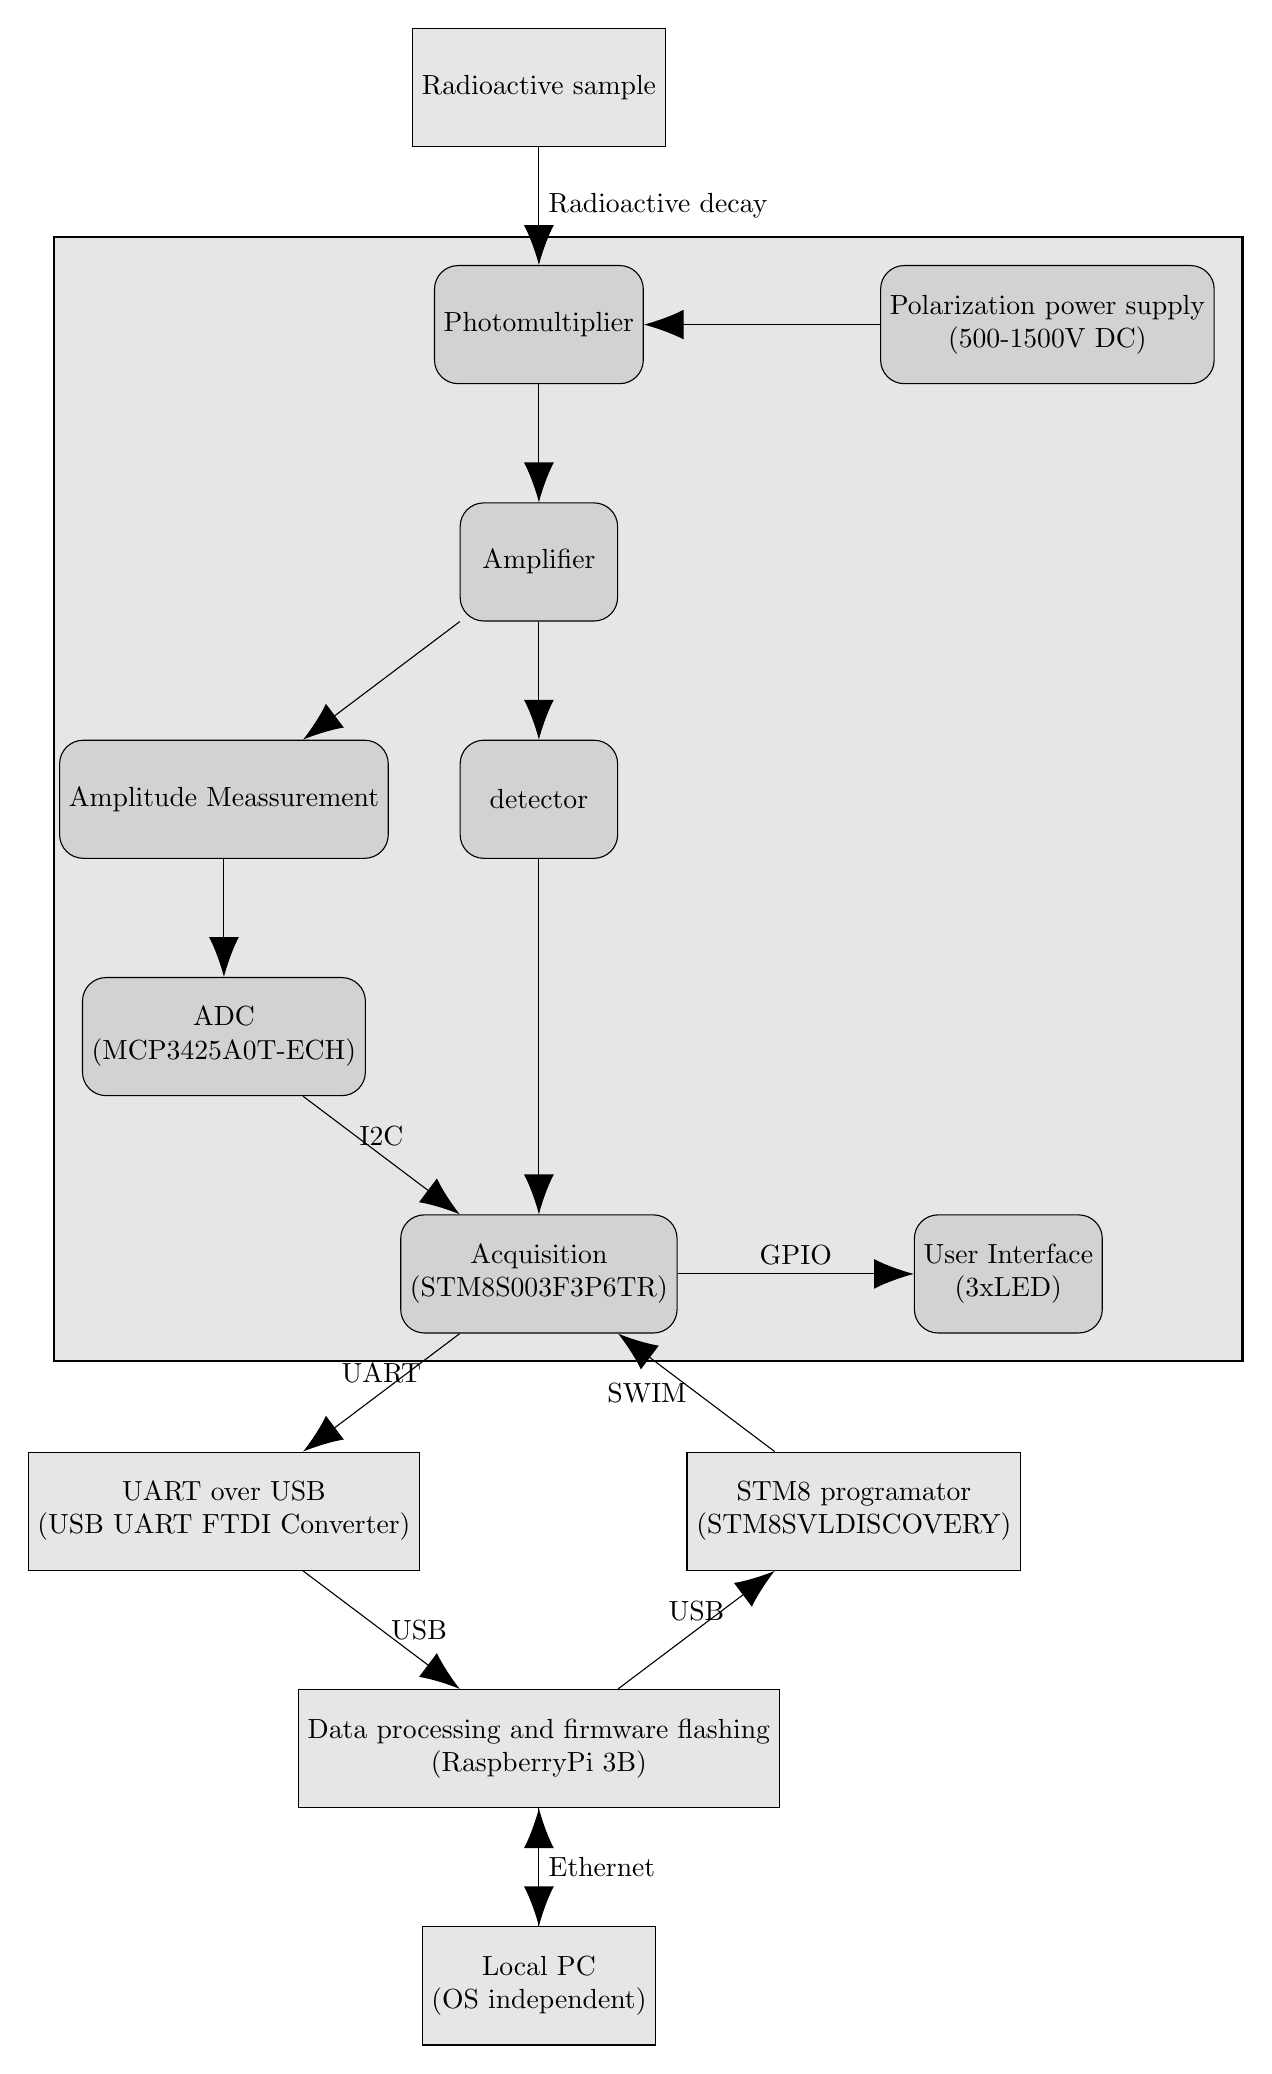
\begin{tikzpicture}[node distance=1.5cm and 3cm]
	% Nodes
	\pgfdeclarelayer{background}
	\pgfsetlayers{background,main}
	
		\node (photomultiplier) [component] {Photomultiplier};
		\node (sample) [system, above=of photomultiplier] {Radioactive sample};
		
		\node (hwpower) [component, right=of photomultiplier] {Polarization power supply\\ (500-1500V DC)};
		\node (amplifier) [component, below=of photomultiplier] {Amplifier};
		
		
		\node (peakssurement) [component, below=of amplifier, xshift=-4cm] {Amplitude Meassurement};
		\node (detector) [component, below=of amplifier] {detector};
		\node (adc) [component, below=of peakssurement] {ADC\\  (MCP3425A0T-ECH)};
		\node (cpu) [component, below=of adc, xshift=4cm] {Acquisition\\ (STM8S003F3P6TR)};
		\node (gui) [component, right=of cpu] {User Interface\\ (3xLED)};
		
		\node (uartconverter) [system, below=of cpu, xshift=-4cm] {UART over USB\\ (USB UART FTDI Converter)};
		\node (stm8programmer) [system, below=of cpu, xshift=4cm] {STM8 programator\\ (STM8SVLDISCOVERY)};
		
		\node (pi) [system, below=of uartconverter, xshift=4cm] {Data processing and firmware flashing\\ (RaspberryPi 3B)};
		\node (pc) [system, below=of pi] {Local PC\\ (OS independent)};
		
		\begin{pgfonlayer}{background}
		\node[system, draw, thick, inner xsep=1em, inner ysep=1em, fit= (photomultiplier) (hwpower) (amplifier) (adc) (cpu)] {};
		\end{pgfonlayer}
		
		% Connectors
		\begin{scope}[->]
		
		\draw [-{Latex[scale=3.0]}] (sample) -- node[anchor=west, minimum width=.25cm, draw=none] {Radioactive decay} (photomultiplier);
		\draw [-{Latex[scale=3.0]}] (hwpower) -- node[anchor=south, minimum width=.25cm, draw=none] {} (photomultiplier);
		\draw [-{Latex[scale=3.0]}] (photomultiplier) -- node[anchor=south, minimum height=.25cm, draw=none] {} (amplifier);
		\draw [-{Latex[scale=3.0]}] (amplifier) -- node[anchor=south, minimum height=.25cm, draw=none] {} (peakssurement);
		\draw [-{Latex[scale=3.0]}] (amplifier) -- node[anchor=south, minimum height=.25cm, draw=none] {} (detector);
		\draw [-{Latex[scale=3.0]}] (peakssurement) -- node[anchor=south, minimum height=.25cm, draw=none] {} (adc);
		\draw [-{Latex[scale=3.0]}] (detector) -- node[anchor=south, minimum height=.25cm, draw=none] {} (cpu);
		\draw [-{Latex[scale=3.0]}] (cpu) -- node[anchor=south, minimum height=.25cm, draw=none] {UART} (uartconverter);
		\draw [-{Latex[scale=3.0]}] (cpu) -- node[anchor=south, minimum height=.25cm, draw=none] {GPIO} (gui);
		\draw [-{Latex[scale=3.0]}] (adc) -- node[anchor=south, minimum height=.25cm, draw=none] {I2C} (cpu);
		\draw [-{Latex[scale=3.0]}] (stm8programmer) -- node[anchor=east, minimum height=.25cm, draw=none] {SWIM} (cpu);
		\draw [-{Latex[scale=3.0]}] (pi) -- node[anchor=south, minimum height=.25cm, draw=none] {USB} (stm8programmer);
		\draw [-{Latex[scale=3.0]}] (uartconverter) -- node[anchor=west, minimum height=.25cm, draw=none] {USB} (pi);
		\draw [-{Latex[scale=3.0]}] (pi) -- node[anchor=west, minimum height=.25cm, draw=none] {Ethernet} (pc);
		\draw [-{Latex[scale=3.0]}] (pc) -- node[anchor=west, minimum height=.25cm, draw=none] {} (pi);
	
	\end{scope}

\end{tikzpicture}
\end{document}
